\documentclass[10pt]{beamer}
\usetheme{AGH}

\usepackage{lmodern}
\usepackage[utf8]{inputenc}
\usepackage{listings} 
\usepackage{siunitx}
\usepackage{filecontents,hyperref}
\usepackage{graphicx}
\usepackage{subcaption}
\usepackage{svg}
\usepackage{appendixnumberbeamer}
\usepackage{booktabs}
\usepackage{xspace}
\newcommand{\themename}{\textbf{\textsc{metropolis}}\xspace}

\definecolor{darkgreen}{rgb}{0.09, 0.45, 0.27}

\title{Status of work on the GGSS system}
\subtitle{\normalsize{Tasks undertaken as part of the engineering and master's thesis}}
\date{17\textsuperscript{th} February 2020}
\author{\normalsize{Arkadiusz Kasprzak \newline \and Jarosław Cierpich \newline \and Grzegorz Podsiadło \newline \newline \and Supervisor: Bartosz Mindur}}



\lstdefinestyle{custom}{
  breaklines=true,
  frame=single,  
  language=[ISO]C++,
  basicstyle=\ttfamily\tiny,
  keywordstyle=\color{blue},
  commentstyle=\color{orange},
  numbers=left,                  
  numbersep=5pt,   
  literate={ą}{{\k{a}}}1
           {Ą}{{\k{A}}}1
           {ę}{{\k{e}}}1
           {Ę}{{\k{E}}}1
           {ó}{{\'o}}1
           {Ó}{{\'O}}1
           {ś}{{\'s}}1
           {Ś}{{\'S}}1
           {ł}{{\l{}}}1
           {Ł}{{\L{}}}1
           {ż}{{\.z}}1
           {Ż}{{\.Z}}1
           {ź}{{\'z}}1
           {Ź}{{\'Z}}1
           {ć}{{\'c}}1
           {Ć}{{\'C}}1
           {ń}{{\'n}}1
		   {Ń}{{\'N}}1
}


\begin{document}

\titleframe[en]

\begin{frame}
\frametitle{Agenda}
\tableofcontents
\end{frame}

\section {New project architecture and migration to GIT}

\begin{frame}{New project architecture}
Characteristics of the new project architecture:
\begin{itemize}
	\item Every module does only need minimal required dependencies to compile
	\item New architecture does bring valuable information about dependencies in the project and inter-module interactions
	\item Modules has been hierarchized. There are hierarchy levels and dependencies point only towards the lower level of hierarchy.
\end{itemize}
\end{frame}

\begin{frame}{New project architecture}
\begin{figure}
\centering
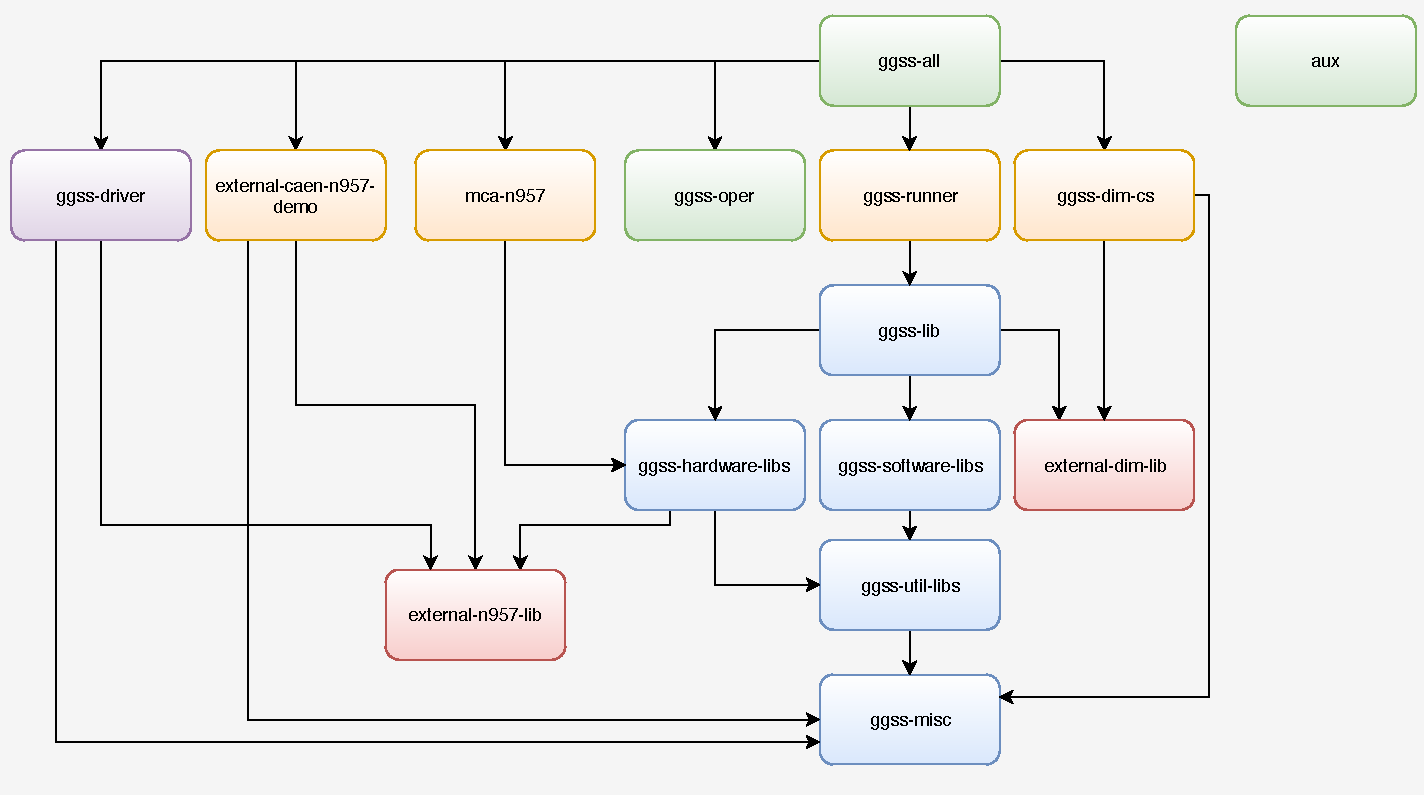
\includegraphics[width=\linewidth]{resources/topLevelArchitecture}
\caption{Architecture of the GGSS project}
\end{figure}
\end{frame}


\begin{frame}{Migration to GIT}
\begin{itemize}
	\item Project has been migrated to GIT version control system. Every module has been divided into separate repository. Submodule feature has been used to achieve hierarchical structure and support fast setup of development environment.
	\item \textbf{atlas-trt-dcs-ggss} group has been created within which 20 repositories has been created.
	\item Issues, Milestones and Kanban Board are being used to organize and track work throughout development.
\end{itemize}
\end{frame}


\section {New building system}

\begin{frame}{New building system}
\begin{itemize}
  \item New system based on CMake has been created.
  \item Hierarchical, information about dependencies clearly visible.
  \item Contains helper Python scripts - for example, in top repository, where user can choose which version should be built.
  \item System can easily be upgraded if some new requirements appear.
\end{itemize}
\end{frame}


\section {Gitlab CI/CD}

\begin{frame}{Gitlab CI/CD}
\begin{minipage}{0.65\linewidth}
\begin{itemize}
  \item Continous Integration and Delivery environment has been created using Gitlab CI/CD.
  \item Building process of applications (ggssrunner, mca-n957 etc.) has been automated. 
  \item Versions: static debug, static release, dynamic debug and dynamic release. 
  \item Product can be downloaded using artifacts system.
\end{itemize}
\end{minipage}
\begin{minipage}{0.32\linewidth}
\begin{figure}
\centering
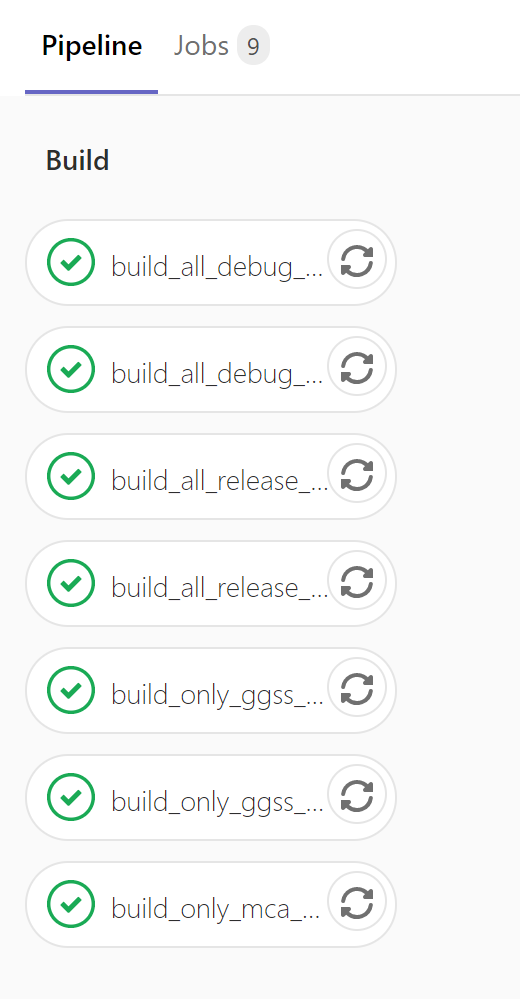
\includegraphics[width=0.8\linewidth]{resources/runnerPipeline}
\caption{Pipeline used for the GGSS runner repository}
\end{figure}
\end{minipage}
\end{frame}

\begin{frame}{Resources}
\begin{minipage}{0.65\linewidth}
	Following resources has been used to establish building environment:
	\begin{itemize}
		\item GitLab CERN resources - to run CI/CD on every single repository except ggss-driver which requires control over installed kernel version
		\item OpenStack CERN resources - to run CI/CD for ggss-driver
	\end{itemize}
	Docker image has been prepared to achieve fast and reliable environment.
\end{minipage}
\begin{minipage}{0.32\linewidth}
	\begin{figure}
		\centering
		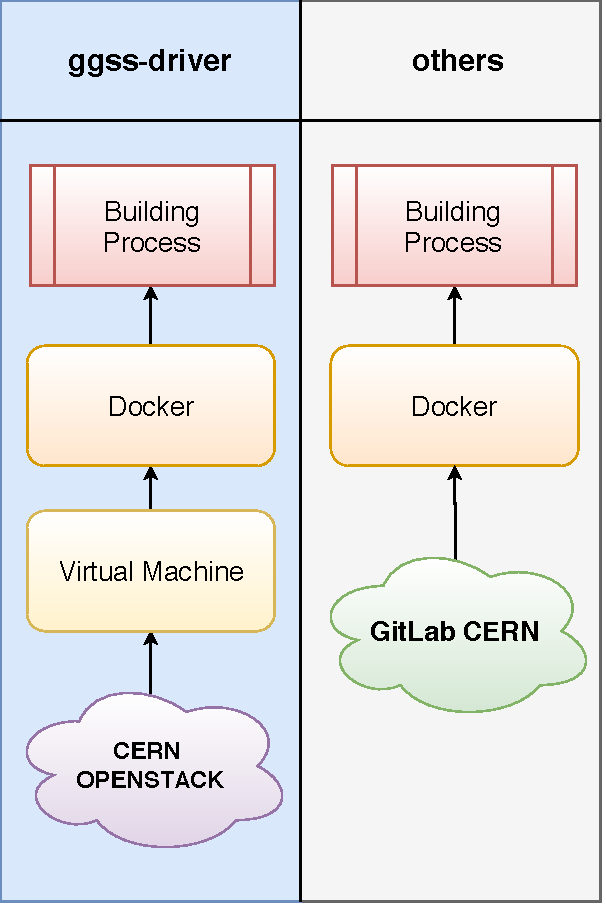
\includegraphics[width=\linewidth]{resources/buildComp}
	\end{figure}
\end{minipage}
\end{frame}

\section {Documentation}

\begin{frame}{Documentation}
\begin{itemize}
  \item Documentation in english is being prepared.
  \item Readme files.
  \item Contains guidelines on how to build every component of the project.
\end{itemize}
\begin{figure}
    \centering
    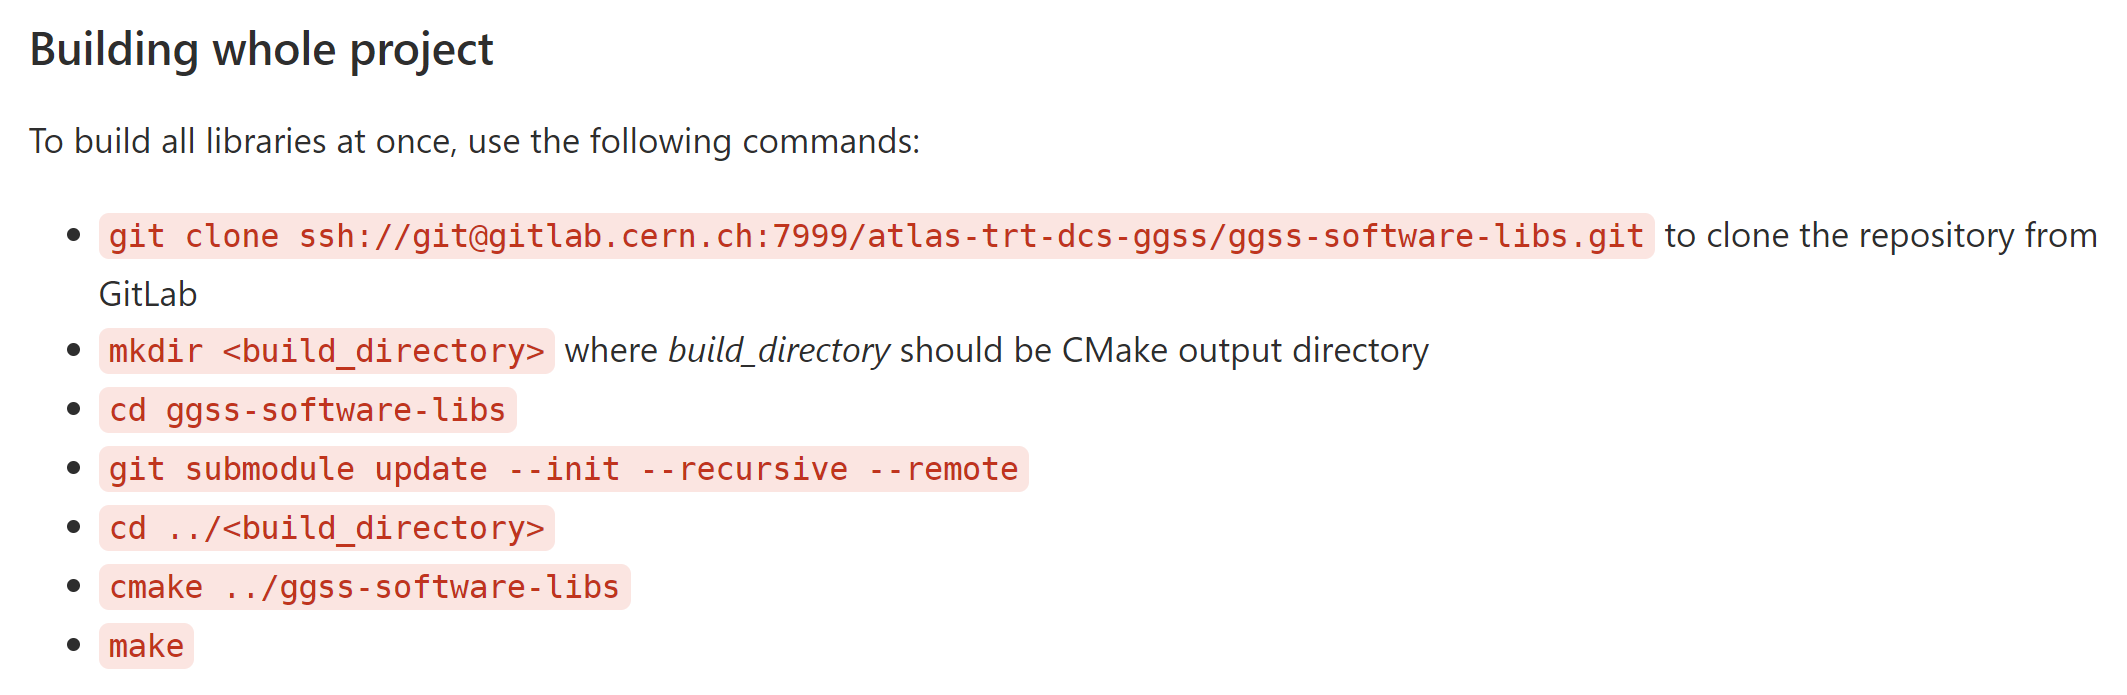
\includegraphics[width=\linewidth]{resources/documentation}
    \caption{Part of documentation that can be found in \textit{ggss-software-libs} repository}
\end{figure}
\end{frame}

\section {Hardware tests}

\begin{frame}{GGSS and hardware tests}
\begin{itemize}
	\item GGSS project has been tested after changes to architecture and building system. Tests were \color{darkgreen}successful\color{black}.
	\item Python scripts were prepared to find and recognize all of connected hardware and test each hardware separately (High Voltage PSU, Multiplexer). Script for hardware discovery can be used separately, it is also included in test scripts.
	\item These scripts, together with application dedicated to Multi Channel Analyzer test, were used to test hardware connection with evaluation machine (pcatltrteval) both via USB Hub and directly. Tests were \color{darkgreen}successful\color{black}.
\end{itemize}
\end{frame}

\section {GGSS Reader and WinCC OA project changes for GGSS}

\begin{frame}{GGSS Reader}
The GGSS Reader is a new tool that simplifies work on WinCC OA project development.
Software allows to simulate the operation of GGSS using old measurements without the need for using hardware.
GGSS Reader comes with the documentation and configured CI.
\begin{figure}
    \centering
    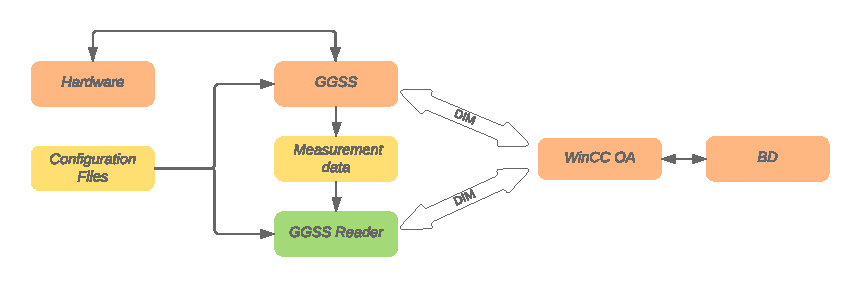
\includegraphics[width=\linewidth]{resources/ggss_reader}
    \caption{Infractructure related to GGSS.}
\end{figure}
\end{frame}

\begin{frame}{WinCC OA project changes for GGSS}
A new spectrum plotting panel was created, which allowed to get rid of external dependencies (gnuplot).
\begin{figure}[H]
  \centering
  \begin{subfigure}[t]{0.48\textwidth} 
      \centering
      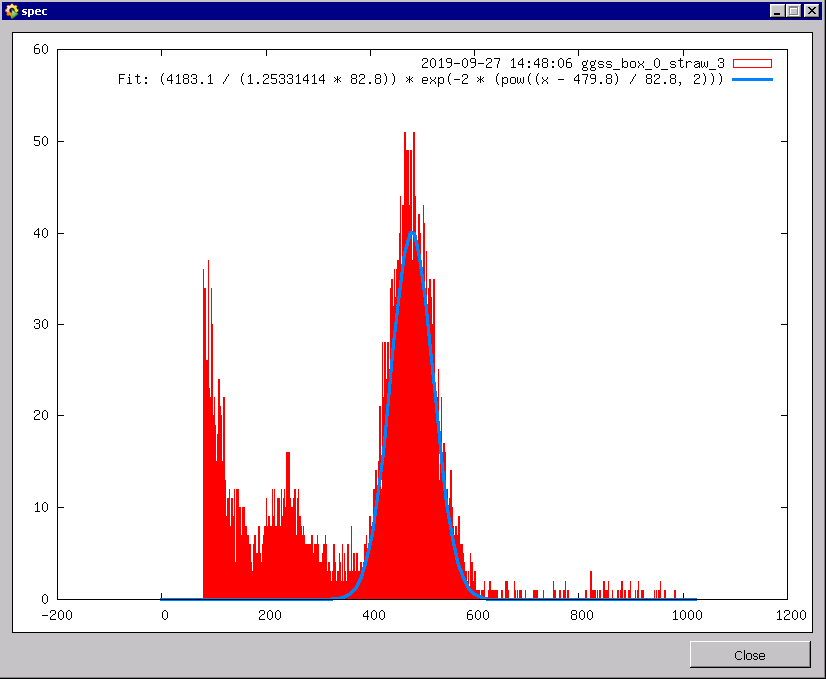
\includegraphics[height=1.6in]{resources/old_spectrum.png} 
      \caption{Old version.} 
  \end{subfigure}
  ~~
  \begin{subfigure}[t]{0.48\textwidth}
      \centering
      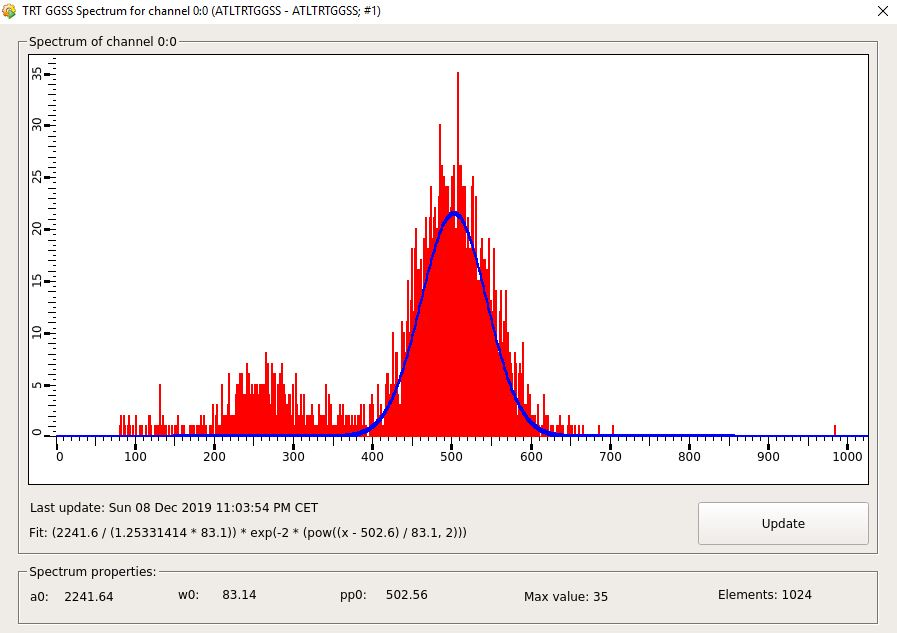
\includegraphics[height=1.6in]{resources/new_spectrum.jpg} 
      \caption{Current version.} 
  \end{subfigure}
    
  \caption{Comparison of spectrum plotting panels.}

\end{figure}


\end{frame}

\section {Plans for future improvements}

\begin{frame}{Plans for future improvements}
\begin{itemize}
\item Automated versioning (master branches version align)
\item Possibility to reuse Continuous Delivery mechanism with debug builds (possibility to use different branch than master to build project)
\item Code refactoring (for example, include paths).
\item Extended GGSS responsiveness - system parameters updated on demand and at the beginning of execution.
\item Improvements in curve fitting algorithm.
\item More options for the GGSS Reader program and a graphical interface for easier data selection.
\end{itemize}
\end{frame}


\begin{frame}
\centering{\huge{Thank You! Questions?}}
\end{frame}

\end{document}